\documentclass[border=0.8ex,svgnames,tikz]{standalone}
\usepackage{amsmath,mathtools}
\usepackage{fontspec}
\setmainfont{Source Serif 4}
\setsansfont{Source Sans 3}
\setmonofont{Source Code Pro}

\usetikzlibrary{positioning,calc}

\begin{document}
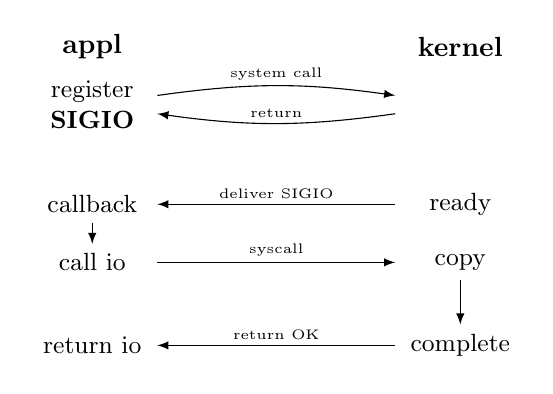
\begin{tikzpicture}
  \coordinate(appl) at (0,0);
  \coordinate(kernel) at ($(appl)+(13.3em,0)$);
  \begin{scope}[
    every node/.style={
      align=center,
      anchor=center,
      font=\small,
      text width=4em,
    },
    ]
    \path[draw=none] node(signal){}
    ++(0,-3.6em) node(ready){ready}
    ++(0,-2.1em) node(copy){copy}
    ++(0,-3.0em) node(complete){complete};
    \node (register)   at ($(signal)-(kernel)-(appl)$)    {register \bf{SIGIO}};
    \node (callback)   at ($(ready)-(kernel)-(appl)$)     {callback};
    \node (call-io)    at ($(callback)+(copy)-(ready)$)   {call io};
    \node (return-io)  at ($(call-io)+(complete)-(copy)$) {return io};
  \end{scope}
  \begin{scope}[
    every node/.style={above,inner sep=0.45ex,font=\tiny},
    every path/.style={draw,>=latex},
    ]
    \path[->]
    (register) edge[bend left=8] node{system call}   (signal)
    (signal)   edge[bend left=8] node{return}        (register)
    (ready)    edge              node{deliver SIGIO} (callback)
    (callback) edge                                  (call-io)
    (call-io)  edge              node{syscall}       (copy)
    (copy)     edge                                  (complete)
    (complete) edge              node{return OK}     (return-io);
  \end{scope}
  \node[above=1ex of register,inner sep=0ex](appl-label){\bfseries appl};
  \node at ($(appl-label)+(kernel)-(appl)$) {\bfseries kernel};
\end{tikzpicture}
\end{document}
